\documentclass[a5paper]{article}
\usepackage[a5paper, top=8mm, bottom=8mm, left=8mm, right=8mm]{geometry}

\usepackage{polyglossia}
\setdefaultlanguage[babelshorthands=true]{russian}

\usepackage{fontspec}
\setmainfont{FreeSerif}
\newfontfamily{\russianfonttt}[Scale=0.7]{DejaVuSansMono}

\usepackage[font=scriptsize]{caption}

\usepackage{amsmath}
\usepackage{amssymb,amsfonts,textcomp}
\usepackage{color}
\usepackage{array}
\usepackage{hhline}
\usepackage{cite}

\usepackage[hang,multiple]{footmisc}
\renewcommand{\footnotelayout}{\raggedright}

\PassOptionsToPackage{hyphens}{url}\usepackage[xetex,linktocpage=true,plainpages=false,pdfpagelabels=false]{hyperref}
\hypersetup{colorlinks=true, linkcolor=blue, citecolor=blue, filecolor=blue, urlcolor=blue, pdftitle=1, pdfauthor=, pdfsubject=, pdfkeywords=}

\usepackage{tabu}

\usepackage{graphicx}
\usepackage{indentfirst}
\usepackage{multirow}
\usepackage{subfig}
\usepackage{footnote}
\usepackage{minted}

\sloppy
\pagestyle{plain}

\title{Domain-Driven Design}
\author{Юрий Литвинов\\\small{yurii.litvinov@gmail.com}}

\date{22.03.2018г}

\begin{document}

\maketitle
\thispagestyle{empty}

\section{Введение}

В этой лекции будет продолжение рассказа про Domamin-Driven Design, а конкретно, про ``тактические'' его аспекты --- идеи и паттерны, близкие к реализации.

Про Domain-Driven Design немного говорилось в прошлый раз, напомню основные моменты:

\begin{itemize}
    \item Domain-Driven Design (или предметно-ориентированное проектирование) --- популярная методология проектирования ПО, которая основана на анализе предметной области и реализации модели предметной области в приложении. Архитектуру в рамках этой методологии предлагается строить не исходя из сиюминутных потребностей реализации, а вокруг ``смыслового ядра'', которое отражает основные сущности реального мира, с которым будет работать программа (или семейство программ).
    \item Модель предметной области выражается прежде всего в коде --- сущности предметной области становятся классами языка программирования, используемого для реализации. Также для обсуждения предметной области с экспертами, а также для документирования модели, часто используются диаграммы.
    \item Немаловажную роль как в создании модели, так и в её ``фиксации'' и улучшении играет ещё и устное общение. Неудачные названия классов или методов, неуклюжие и непонятные описания взаимодействий прекрасно слышны в разговоре и являются поводом для того, чтобы посмотреть на модель ещё раз. Сам естественный язык часто подсказывает правильные архитектурные решения --- что неудивительно, язык сотни лет оттачивался как раз для того, для чего он нужен в DDD --- для передачи сути понятий. Ещё раз напомню, что архитектура --- это больше про понимание программы человеком, а не понимание программы компьютером, так что всякие гуманитарные вещи могут сильно помочь при разработке архитектуры.
    \item Модель определяет единый язык, на котором должны общаться все члены команды и эксперты предметной области, которые им помогают. Если какой-то термин зафиксирован как имя класса, использование его синонимов ни в диалогах, ни в документации, ни тем более в коде не допускаются, можно использовать только имя класса. Так же и с методами --- если действию дали название, можно использовать только его, и если это не удобно, название меняют. Это, во-первых, упрощает общение и сопровождение программы, во-вторых, способствует улучшению модели, постоянно её тестируя на предмет неконсистентностей, недопониманий и неоднозначностей.
    \item Модель появляется не только благодаря применению единого языка и последовательного именования всех нужных сущностей, она также ``выкристаллизовывается'' в процессе непрерывного рефакторинга и уточнения. Поскольку программисты редко владеют предметной областью, в которой они решают задачу, построить правильную и хорошую модель предметной области невозможно просто потому, что знаний не хватает. Есть понятие ``переработка знаний'' --- когда программисты строят модель, одновременно активно изучая предметную область. Узнав что-то новое, они включают это в модель, рисуют диаграммы, обсуждают их с экспертами, корректируют модель, и т.д. до тех пор, пока не будет достигнуто достаточное понимание. Цель ``переработки знаний'' --- не получить понимание, достаточное для реализации программы, а понять принципы, по которым работает сама предметная область, а уже потом написать программу. Интересно, что если модель хороша и программисты неплохи в выделении абстракций, то в процессе переработки знаний кое-чему научиться могут и эксперты.
\end{itemize}

Дальнейший рассказ является, по сути, кратким пересказом книги Эрик Эванс, ``Предметно-ориентированное проектирование. Структуризация сложных программных систем''. М., ``Вильямс'', 2010, 448 стр., по крайней мере, первых трёх её частей. Если есть время, лучше её прочитать, если нет, то по этому конспекту, я надеюсь, можно составить общее представление. Некоторые примеры и все картинки взяты оттуда.

\section{Единый язык}

Единый язык --- одно из ключевых понятий предметно-ориентированного проектирования. Необходимость его введения связана с тем, что программисты и специалисты предметной области разговаривают на разных профессиональных жаргонах и изначально не понимают друг друга. Если программисты будут общаться в терминах реализации, экспертам это будет не очень полезно. Причём, что особенно опасно, непонимание будет, скорее всего, скрытым --- они будут чувствовать себя, как типичные студенты на лекции по матанализу: вроде общий смысл улавливается, но местами происходит что-то такое, с чем, кажется, можно будет разобраться потом, прочитав конспект. Но лекцию по матанализу ведёт человек, разбирающийся в предмете, а обсуждающий с заказчиком программу программист, возможно, просто неправ, или подсознательно маскирует своё собственное непонимание техническими терминами, отчего и эксперт его не понимает, но не может поправить.

На самом деле, даже среди разработчиков одной группы вырабатывается свой жаргон, который может быть непонятен новичкам и даже опытным членам соседних групп, работающих над тем же проектом. Это плохо, во-первых, тем, что необходимость постоянно переводить понятия с одного языка на другой вызывает ``размытие'' этих понятий и некоторую неопределённость, причём, каждый может делать перевод по-своему, что усиливает хаос. Во-вторых, это плохо тем, что один термин может использоваться в разных (иногда очень слегка разных) значениях --- внутри проекта возникают ``ереси'', что приводит уже к откровенной путанице и багам в коде.

Поэтому предметно-ориентированное проектирование предписывает выработку единого языка и использование его повсюду в проекте, от составления технического задания до имён методов, переменных и тестов. В единый язык входят термины предметной области --- как правило, они становятся именами классов, отношения между понятиями и действия, которые сущности могут выполнять --- это имена методов, также в язык попадают имена паттернов, используемых при проектировании системы, даже если их в предметной области нет (например, ``репозиторий'' или ``спецификация''). Ещё единый язык должен содержать понятия, относящиеся к высокоуровневой архитектуре системы, которые напрямую невыразимы в коде --- уровни, ограничения на взаимодействие (например, понятие ``канал'' в архитектурном стиле ``каналы и фильтры'' может явно в коде никак не выражаться, но в архитектуре играет ключевую роль).

Единый язык не создаётся мгновенно, он эволюционирует вместе с пониманием предметной области, моделью и кодом, который эту модель реализует. Поэтому за изменениями языка, которые возникают естественно в разговорах (а помним, что общаться можно только на едином языке), надо следить и соответственно рефакторить модель или код. Например, если все начали говорить ``связь'' вместо ``ассоциация'' (потому что так короче и благозвучнее), надо переименовать соответствующий класс и в коде.

На самом деле единых языков в проекте может быть много, как бы бредово это ни звучало. Если проект состоит из нескольких более-менее обособленных частей, то почему нет, каждая из них может иметь свой язык. Например, система планирования грузоперевозок вполне может использовать библиотеку алгоритмов на графах, в самой системе связь может называться ``перевозка'', а в библиотеке --- ``ребро''. Если есть чёткая граница между сферами действия разных языков (и разных моделей и даже мировоззрений, которые связаны с языком) и определены правила преобразования одного в другое (выражающиеся в коде в виде фасадов и адаптеров), то почему нет, это помогает уменьшить общую сложность системы. Если чёткой границы нет и модели (и языки) начинают проникать друг в друга, возникает путаница, которая может привести к провалу проекта.

Небольшой пример важности единого языка. Положим, нам надо сделать систему планирования грузоперевозок и мы рассматриваем задачу прокладки маршрута перевозки через какой-то пункт таможенного контроля. Мы везём груз из точки А в точку Б через 0 или больше пунктов таможни, и у нас есть планирвощик маршрута, которому можно сказать точки А, Б и таможни, чтобы он выдал расписание перевозки. Модель глазами программиста могла бы выглядеть так:

\begin{center}
    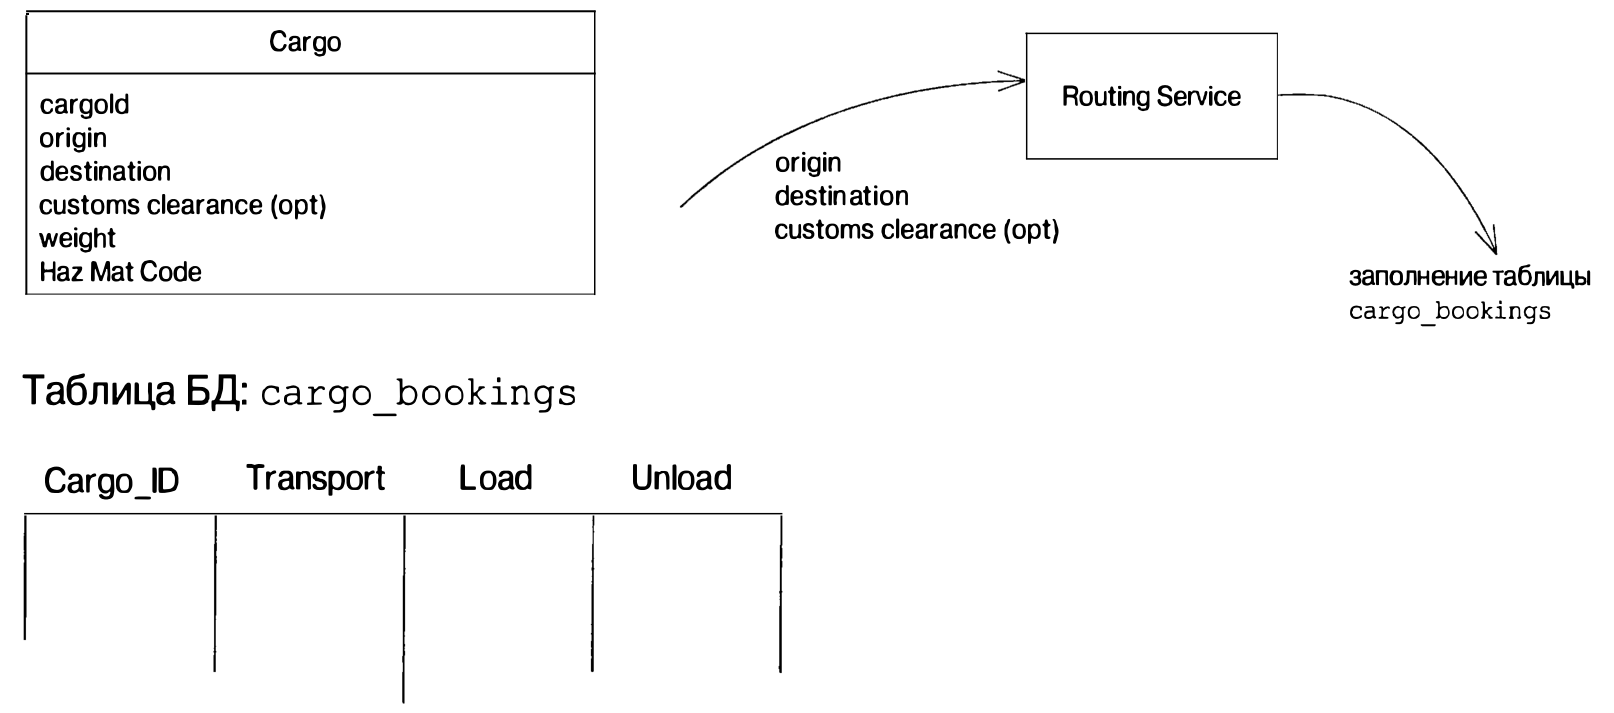
\includegraphics[width=0.9\textwidth]{lowAbstractionLanguage.png}
\end{center}

Представьте себе обсуждение с экспертом по логистике вопроса изменения пункта растомаживания:

\textit{``Тогда мы удаляем все строки в таблице отправки грузов с задан­ным идентификатором груза, потом передаем пункт отправки, пункт назначения и новый пункт растаможивания в Маршрутизатор (Routing Service) и он заполняет таблицу заново. В объект Груз (Cargo) надо добавить логический переключатель, указывающий, есть ли данные в таблице отправки.''}

Сравним это с вот такой моделью:

\begin{center}
    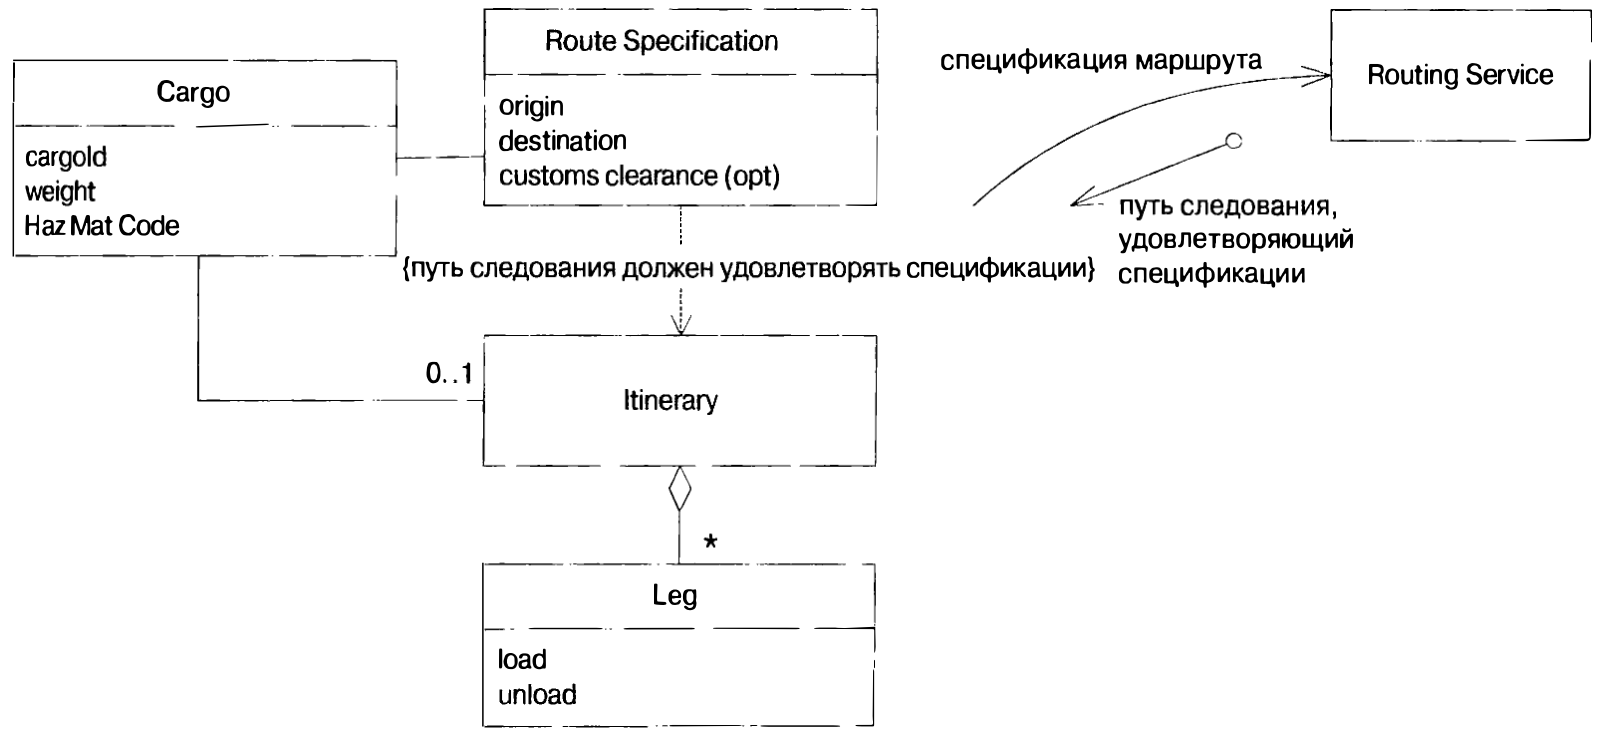
\includegraphics[width=0.9\textwidth]{highAbstractionLanguage.png}
\end{center}

Тут наше обсуждение могло бы выглядеть так:

\textit{``При изменении любого из атрибутов в Спецификации маршрута (Route Specification) мы удаляем старый Маршрут (Route) и просим Маршрутизатор (Routing Service) построить новый маршрут на основе новой Спецификации маршрута.''}

Получилось короче, более точно и даже более полно, потому что в модели выше надо было ещё пояснять, когда сбрасывать маршрут, а тут появилось понятие ``Спецификация маршрута''. Вторая модель (и язык, с ней связанный) по сути радикально систему не меняет (Leg и Itinerary всё также могут быть таблицами в БД), оставляет гораздо меньше возможностей для взаимного непонимания и ошибок, с ним связанных.

Ещё один хороший пример использования единого языка, из книжки:

\begin{center}
    \textit{Если передать в \textbf{Маршрутизатор} пункт отправки, пункт назначения, время прибытия, то он найдет нужные остановки в пути следования груза, а потом, ну... запишет их в базу данных.}

    \vspace{4mm}

    \textit{Пункт отправки, пункт назначения и все такое... все это идет в \textbf{Маршрутизатор}, а оттуда получаем \textbf{Маршрут}, в котором записано все, что нужно.}

    \vspace{4mm}

    \textit{\textbf{Маршрутизатор} находит \textbf{Маршрут}, удовлетворяющий \textbf{Спецификации маршрута}.}
\end{center}

Опять-таки, видно, что хорошая модель позволяет строить фразы коротко, точно и без технических подробностей. Но тут ещё видно, как естественный язык помогает процессу разработки архитектуры --- мы начали с первой фразы, запнулись, потому что у нас не было сущности ``Маршрут'', добавили её в модель, стало лучше, но теперь нам не нравится ``и всё такое'', что мы побеждаем добавлением понятия ``Спецификация маршрута''. Конечно, натуральный язык и метафоры могут завести не туда, но если это случится, то это скорее проблемы понимания предметной области, и их будет проще найти, чем если бы эти проблемы были бы спрятаны в таблицах в базе данных.

\section{Модель и реализация}

Модель предметной области полезна только в том случае, если она непосредственно связана с кодом. Бывает так, что люди, вообразившие себя крутыми архитекторами, рисуют огромную модель предметной области в виде диаграммы классов UML, которую невозможно эффективно реализовать, например, положить в базу данных. Тогда обычно разработчикам приходится частично игнорировать модель, решая свои чисто практические задачи. Это приводит к тому, что код и модель расходятся, при этом модель становится даже вредна, поскольку врёт об устройстве кода.

Бывает и наоборот, люди, вообразившие себя крутыми agile-developer-ами, начинают ``фигачить код'' безо всякой архитектуры-шмархитектуры. В результате получается программа, полученая хаотичным наслоением слабо связанной функциональности, которую тяжело читать, сопровождать, добавлять новую функциональность. Эванс в книжке кратко описывает два таких проекта и делает интересное наблюдение, что результаты получились примерно одинаковыми.

Из этого следует вывод, что модель всегда должна быть связана с кодом, а добиться этого можно только если каждый архитектор пишет код и любой программист участвует в моделировании. Практика, принятая в некоторых enterprise-проектах, когда аналитики сначала строят модель предметной области, а затем программисты её реализуют, пагубна именно поэтому --- модель может игнорировать особенности реализации, а знания аналитиков не будут полностью переданы программистам. И наоборот, новые интересные знания могут быть получены при попытке выразить модель в коде, эти знания аналитикам (или архитекторам) не попадут. В результате программистам придётся проделывать работу по анализу предметной области фактически заново, и ``prescriptive architecture'' разойдётся с ``descriptive architecture''. Есть даже хороший термин ``разрушительный рефакторинг'', когда программисты, не понимая глубоко предметную область, рефакторят программу так, чтобы было удобно реализовывать требуемую функциональность. В этот момент, скорее всего, потеряется самая суть программы, её смысловое ядро, и это будет просто работающее приложение, которое будет делать что нужно. DDD же ставит своей целью создавать системы, которые делают больше и лучше, чем нужно (при этом будучи менее трудозатратными при разработке).

Поэтому модели в DDD приходится быть одновременно и моделью анализа, и моделью проектирования. Мы с её помощью пытаемся понять предметную область, и она же используется для того, чтобы писать код (причём, одновременно). Так что если модель окажется полной технических деталей, то анализ предметной области и общение с экспертами неизбежно пострадают, а если она будет слишком абстрактной или непроработанной, то пострадает реализация. Необходим баланс, который достигается обычно за несколько итераций --- описываем предметную область, пытаемся её реализовать, получается плохо, правим модель и рефакторим код, пытаемся описать предметную область в новой модели, получается неуклюже, снова рефакторим модель и т.д., пока не придём к модели, которая хорошо служит и коду, и объяснению предметной области. 

При этом, разумеется, необходимо, чтобы выбранный язык программирования поддерживал парадигму моделирования --- например, с ООП всё довольно легко, а вот с чисто структурными языками, например, C, может быть плохо --- в них не выразить естественным образом сущности с состоянием и поведением, свойственные реальному миру. А вот Prolog, напротив, хорош, он близок исчислению предикатов, так что если мы можем построить модель в терминах фактов и правил вывода, на Прологе программа запишется очень естественно.

Ещё не рекомендуется разделять модель, которая служит основой реализации, и модель, которую показывают пользоателю. Пример --- в Internet Explorer закладки хранились как файлы-ярлыки на диске, но пользователю про это ничего не говорилось. Хочет пользователь сохранить закладку с символом ``:'', а ему ошибка --- неправильное имя файла. И пользователь не может понять, какого к чёрту файла, он просто закладку сохранил. А вот если бы закладки и показывались как файлы, то пользователь мог бы сортировать их с помощью файлового менеджера или вообще скрипта, и был бы более счастлив.

\section{Изоляция предметной области}

Хорошо, допустим, мы смогли построить модель предметной области. Но этого недостаточно, чтобы получить работающую программу --- нужен ещё пользовательский интерфейс, сеть, база данных, всякого рода вспомогательный код, логирование, обработка ошибок, юнит-тесты и т.д. Основная идея DDD в том, что всё это должно быть архитектурно отделено от модели предметной области, чтобы код модели --- код, в котором сосредоточена вся суть приложения --- мог быть максимально простым, небольшим по размеру и содержащим только существенные для смысла системы вещи. Всё остальное должно находиться в отдельных модулях и просто использовать классы доменной модели.

Самый популярный способ достижения такого разделения (хотя и не единственный) --- уровневая архитектура. Программа реализуется в виде набора уровней, где каждый уровень может непосредственно взаимодействовать только с уровнями ниже. Способов разделения на уровни бывает много (трёхзвенная архитектура, семь уровней OSI, четыре уровня TCP/IP и т.д.), DDD требует лишь, чтобы среди всех уровней был уровень предметной области, на котором и сосредоточены все классы модели.

Довольно типичный для информационных систем способ разделения на уровни представлен на картинке:

\begin{center}
    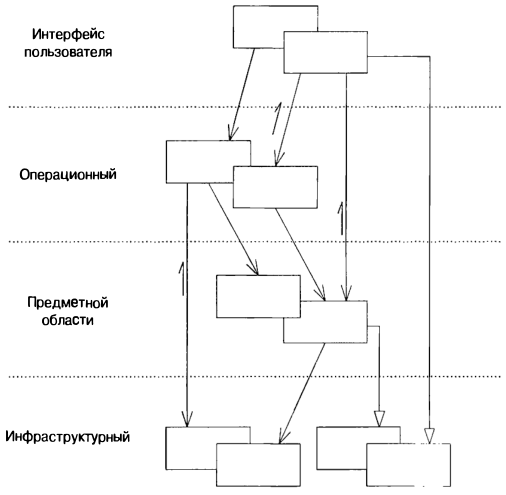
\includegraphics[width=0.6\textwidth]{layers.png}
\end{center}

Уровень интерфейса отвечает только за взаимодействие с пользователем и реализует только отображение и обработку событий. Никакой содержательной логики в нём быть не должно. Операционный уровень (application layer) занимается координацией действий бизнес-объектов, которые находятся на уровне предметной области. Операционный уровень тоже должен быть очень простым, его ответственность --- это инициализировать систему и по сигналу от интерфейса инициировать нужные пользователю операции. Инфраструктурный уровень содержит все вспомогательные вещи, неспецифичные для данной предметной области, например, код работы с базой данных или код работы с сетью.

Уровень предметной области содержит бизнес-объекты, которые ничего интересного кроме, собственно, реализации бизнес-правил, не делают. Их реализация должна быть максимально простой, и именно их реализации следует уделять максимум внимания, потому как именно уровень предметной области определяет конкурентные преимущества и полезность программы.

Операционный уровень специфичен для каждого конкретного приложения, тогда как уровень предметной области может разделяться между несколькими приложениями в семействе. На операционном уровне из классов уровня предметной области собирается то, что делает конкретно наше приложение, операционный уровнь же координирует бизнес-объекты. Но бизнес-регламенты (например, последовательность действий в бизнес-процессе) должны быть реализованы на уровне предметной области, потому как они хоть и координируют действия других объектов, но объективно присутствуют в предметной области и могут быть переиспользованы в других приложениях. Операционному уровню также запрещается иметь состояние (кроме, быть может, состояния, необходимого для общения с пользователем приложения, типа прогресса операций).

Инфраструктурный уровень поддерживает все уровни выше. Он может обеспечивать архитектурную среду для всех остальных уровней (например, Java Beans или ROS), может содержать специфичный для приложения код работы с третьесторонними библиотеками и технологиями (например, Object-Relational Mapping). Может показаться противоестественным, что базовые классы для уровней выше могут быть на инфраструктурном уровне (то есть деревья наследования растут вверх), но если подумать, кто о ком больше знает --- предок или потомок, то становится понятно, что концептуально всё ок.

Уровням ниже, естественно, иногда требуется общаться с уровнями выше. Даже инфраструктурный уровень, если он не состоит только из библиотек, может инициировать действия на уровнях выше (например, получение сетевого пакета вызывает обработку на операционном уровне). Поскольку общаться напрямую уровни не могут, применяются приёмы ``косвенного'' вызова --- callback-и (или виртуальные методы --- hook-и), паттеррн ``Наблюдатель'', ``дедушка всех паттернов'' MVC. Такой подход несколько затрудняет отладку, но позволяет разрабатывать каждый уровень независимо, и не думать, как будут пользоваться кодом уровня другие.

В реальной жизни часто встречается диаметральная противоположность такого подхода --- антипаттерн ``умный GUI''. Это когда вся бизнес-логика приложения реализуется прямо в классах, отвечающих за пользовательский интерфейс, как правило, в обработчиках библиотечных событий. При этом даже работа с БД может выполняться из кода GUI.

Как ни странно, это не всегда плохо. Во-первых, есть куча тулов для быстрой разработки пользовательских интерфейсов, при этом подходе их можно задействовать на полную --- большая часть приложения будет просто сгенерена. Во-вторых, это быстро --- рабочее приложение таким способом можно написать за пару часов, при этом нет оверхеда на создание классов, интерфейсов, наладку общеиня между уровнями, организацию взаимодействия. Легко добавлять в приложение новые фичи --- просто кидаем на форму новый контрол, цепляем к нему новый обработчик, и в продакшн. Причём, поскольку код каждого куска такой функциональности довольно прост, его несложно поддерживать или переписать заново.

Однако если ожидаемый размер проекта превышает где-то 3000 строк кода, ``Умный GUI'' быстро становится антипаттерном. Почему: невозможно проектирование по модели, классов предметной области просто нет, есть методы-обработчики, в которых код интерфейса смешан с бизнес-правилами и инфраструктурным кодом. Поэтому переиспользование бизнес-правил чрезвычайно затруднено, фактически, если две фичи требуют одного бизнес-правила, его надо реализовать дважды. Сложное поведение в такой ситуации оказывается сложно реализовать --- не получится аккуратно декомпозировать его на набор взаимодействующих объектов без разделения на уровни. Практически невозможна интеграция с другими системами --- всё завязано на GUI, так что реализовать отдельный API для интеграции может быть очень сложно (опять-таки, в процессе сами собой появятся бизнес-объекты и уровни, так почему не сделать сразу нормально?).

\end{document}